Galant is a successor to
GDR~\cite{1991-TR_NCSU_CSC-Stallmann,1992-CSDM-Stallmann} and has much of the
same functionality.
The design of GDR is illustrated in Fig.~\ref{fig:gdr}.
To the left of the dotted line are the interactions with external entities,
as supported by GDR.
The GDR user, when running a specific animation created and compiled
externally, acts as both the editor of problem instances and as initiator of an
algorithm animation with which (s)he may then interact, i.e., plays the role
of explorer and of observer. 
Input and output take the form of a simple text-based file format that can be
manipulated outside of GDR via text filters, graph editors, graph drawing
applications, etc. It is this external manipulation capability
that makes GDR a tool rather than a
closed system.

The animation creator writes a C program that interacts with a graph ADT
whose functions access and/or modify both the internal representation of the
graph and the user's view of it. The ADT functions can be classified into one
of three categories depending on the graph attributes accessed:
(i)~\emph{logical} attributes --- labels (and identities) of nodes and labels
and endpoints of edges; (ii)~\emph{geometric} attributes --- the positions of
nodes and labels and
inflection points of edges; and (iii)~\emph{display} attributes ---
highlighting of nodes and edges, making labels visible/invisible, etc. 

\begin{figure}

\begin{center}
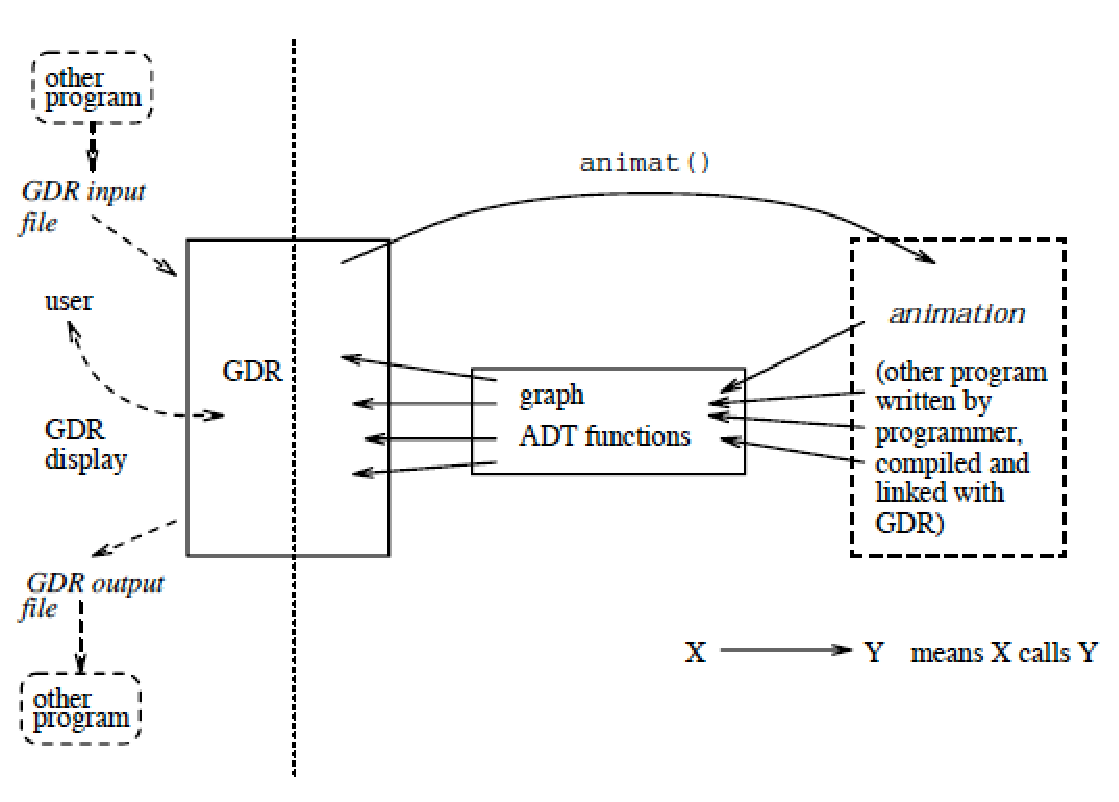
\includegraphics[scale=0.6]{X_gdr_design}
\end{center}

\caption{GDR design.}
\label{fig:gdr}
\end{figure}

While GDR has much to recommend it when compared with other algorithm
animation software, it suffers from some serious drawbacks:

\begin{itemize}
\item
  Each animation is a separate C program that interacts with an X11 window
  server.
  Therefore GDR is not portable.
  %% It is not possible to load (and apply) more than one animation to
  %% the same graph.
\item
  The user interface is crude. Aside from being black and white it has no
  file browser, no rubber-banding of moves, non-standard keyboard shortcuts
  and an unappealing look and feel.
%% \item
%%   The format for storing graphs, while simple and text-based, does not
%%   resemble any other graph format and is difficult to edit or filter.
\item
  While the API supports access to the graph itself, there is no API support for
  data structures commonly used in graph algorithms (stacks, queues, priority
  queues).
\end{itemize}

% [Last modified: 2013 06 25 at 14:51:36 GMT]
